\chapter{التحكم الهرموني في التكاثر}\label{ch:b2:reproductive-hormones}

في كل شهر، وفق جدول يُحفظ في حدود يوم أو يومين طوال ثلاثين
سنة، ينضج \omterm{def:b2:mammal-reproduction:ovary}{جريب} واحد، وتُطلق بويضة واحدة، وتُبنى \omterm{def:b2:reproductive-hormones:cycle}{بطانة
الرحم} ثم تُهدم، ما لم يصل جنين. ولا ساعة في الجسم تدق
بهذا المعدل؛ وإنما ينبثق الإيقاع من محادثة بين ثلاثة أعضاء ---
الوطاء والنخامى والمبيض --- يتحكم فيها كل هرمون في
إطلاق الذي يليه ويتحكم الأخير في الأول. يفكك هذا الفصل
تلك المحادثة: المحور الذي يدير الجنسين، والتحكم المقوّي في \omterm{def:b2:mammal-reproduction:testis}{الخصية}،
والتحكم الدوري في المبيض بانقلابه اللافت من التغذية الراجعة السالبة
إلى الموجبة، والطرق التي يُتجاوز بها المحور بالحمل والأدوية
والعيادة.

\section{المحور}

\begin{definition}[المحور الوطائي--النخامي--المنسلي]\label{def:b2:reproductive-hormones:axis}
\index{الهرمون المطلق لموجهة الغدد التناسلية}\index{الهرمون الملوتن}\index{الهرمون المنبه للجريب}\index{تغذية راجعة سالبة!هرمونية}
تفرز عصبونات \emph{الوطاء} \emph{GnRH}
(الهرمون المطلق لموجهة الغدد التناسلية، وهو ببتيد من عشرة حموض أمينية) في
الأوعية البابية الصغيرة الذاهبة إلى \emph{النخامى الأمامية}،
في \emph{نبضات} قصيرة كل ساعة إلى ساعتين. ويجعل هذا الهرمون
النخامى تفرز هرمونين بروتينيين سكريين في الدوران
العام، وهما \emph{موجهتا الغدد التناسلية} \emph{LH} (الهرمون
الملوتن) و\emph{FSH} (الهرمون المنبه \omterm{def:b2:mammal-reproduction:ovary}{للجريب}). وهذان يؤثران في
\emph{المناسل}: فهرمون LH يؤثر في الخلايا الصانعة للستيرويدات (خلايا لايديغ،
وخلايا القِراب \omterm{def:b2:mammal-reproduction:ovary}{والجسم الأصفر})، وFSH في الخلايا التي ترضع الأعراس
(خلايا سرتولي والحُبيبية). وتجيب المناسل بستيرويدات ---
\emph{التستوستيرون}، و\emph{الإستراديول}، و\emph{البروجستيرون} --- و
بالببتيد \emph{الإنهيبين}، وهذه تغذي راجعًا على
الوطاء والنخامى: الستيرويدات على كليهما، وأكثره
\emph{سالب}؛ والإنهيبين على FSH وحده. والنتيجة حلقة
منظَّمة يُبقى فيها خرج المنسل عند نقطة ضبط، وينظّم
التصميم الثلاثي الطبقات نفسه الدرقيةَ وقشر الكظر. أما
الآليات التي تعمل بها هذه الهرمونات في خلاياها فهي موضوع
\cref{ch:b2:cell-signalling}.
\end{definition}

\begin{omfigure}
\begin{tikzpicture}[every node/.style={font=\scriptsize}, >=stealth]
  \node[draw, rounded corners, fill=omDef!15, align=center, minimum width=3cm] (hyp) at (0,4.2) {الوطاء\\GnRH، في نبضات};
  \node[draw, rounded corners, fill=omDef!15, align=center, minimum width=3cm] (pit) at (0,2.2) {النخامى الأمامية\\LH وFSH};
  \node[draw, rounded corners, fill=omProp!20, align=center, minimum width=3cm] (gon) at (0,0) {المنسل\\ستيرويدات، وإنهيبين};
  \node[draw, rounded corners, fill=omExo!25, align=center, minimum width=3cm] (tar) at (5.2,0) {الأنسجة الهدف\\تكوّن الأعراس، والقنوات،\\والصفات الثانوية};
  \draw[->, thick] (hyp) -- (pit) node[midway, right] {أوعية بابية};
  \draw[->, thick] (pit) -- (gon) node[midway, right] {الدم};
  \draw[->, thick] (gon) -- (tar);
  \draw[->, thick, omThm] (gon.west) .. controls (-3.0,0) and (-3.0,2.2) .. (pit.west);
  \draw[->, thick, omThm] (gon.west) .. controls (-4.6,0) and (-4.6,4.2) .. (hyp.west);
  \node[omThm, anchor=east, align=right] at (-3.9,1.2) {إلى النخامى:\\ستيرويدات $(-)$،\\وإنهيبين $(-)$ على FSH};
  \node[omThm, anchor=east, align=right] at (-3.9,3.6) {إلى الوطاء:\\ستيرويدات $(-)$\\(الإستراديول $(+)$\\في منتصف الدورة)};
\end{tikzpicture}

{\small المحور: يقود GnRH الوطائي هرموني LH وFSH النخاميين،
وهما يقودان المنسل؛ وستيرويدات المنسل وإنهيبينه تغذيان راجعًا
سالبًا على الطبقتين العلويتين --- عدا التغذية الراجعة الموجبة
القصيرة للإستراديول التي تطلق \omterm{def:b2:mammal-reproduction:ovary}{الإباضة}.}
\end{omfigure}

\begin{proposition}[لماذا تهم النبضات]\label{prop:b2:reproductive-hormones:pulses}
\index{إفراز نبضي}\index{تبلّد المستقبل}
لا تستجيب النخامى للهرمون المطلق إلا إذا وصل في نبضات. فالخلية
المعرَّضة لهرمون باستمرار تزيل مستقبلات الهرمون
من سطحها (\emph{التبلّد})؛ فإذا جُدّد مخزون المستقبلات
بمعدل $s$، وأُزيل بمعدل قاعدي $d$، وأُزيل، في
حضور الهرمون $H$، بمعدل إضافي $iH$، كان
\[
\frac{\mathrm{d}R}{\mathrm{d}t} = s - (d + iH)\,R, \qquad R^* = \frac{s}{d + iH},
\]
فيدفع $H$ العالي المستمر عدد المستقبلات إلى حالة مستقرة
منخفضة وتخرس الخلية، في حين تدع النبضات القصيرة المفصولة
بفترات خالية من الهرمون المخزون يتعافى
(بثابت زمن $1/d$) بينها. فنبضة كل تسعين
دقيقة تبقي النخامى مستجيبة؛ أما التسريب المستمر، أو
ناهض طويل الأثر للهرمون المطلق، فيغلقها في غضون أيام --- وهو أساس
الأدوية التي تكبت المحور في سرطان الموثة وفي \omterm{def:b2:reproductive-hormones:cycle}{بطانة الرحم} الهاجرة
وفي البلوغ المبكر. ويرمّز تواتر النبضات معلومة أيضًا:
فالنبضات السريعة تفضّل LH، والبطيئة تفضّل FSH.
\end{proposition}
\begin{proof}[شواهد]
أتلف كنوبيل (1978--1980) عصبونات الهرمون المطلق عند قرود الريسوس،
فألغى ذلك LH وFSH والدورة، ثم عوّض الهرمون المطلق
بمضخة: فأعادت نبضة في الساعة موجهتي الغدد التناسلية ودورات
\omterm{def:b2:mammal-reproduction:ovary}{الإباضة} الطبيعية؛ أما الجرعة اليومية نفسها معطاةً باستمرار فأعادتهما
أيامًا قليلة ثم انهار LH وFSH إلى الصفر؛ والعودة
إلى النبضات أعادتهما من جديد. فنمط التسليم، لا
المقدار، هو الإشارة.
\end{proof}

\begin{omfigure}
\begin{tikzpicture}
\begin{axis}[
  width=0.8\linewidth, height=5.4cm,
  axis x line=bottom, axis y line=left,
  xmin=0, xmax=40, ymin=0, ymax=1.2,
  xlabel={الأيام}, ylabel={LH في البلازما (نسبيًا)},
  xlabel style={font=\small, at={(axis description cs:0.5,-0.13)}, anchor=north},
  ylabel style={font=\small},
  tick label style={font=\small}, xtick={0,10,20,30,40}, ytick={0,0.5,1},
  clip=false,
]
\addplot[very thick, omDef, domain=0:10, samples=2] {1};
\addplot[very thick, omThm, domain=10:25, samples=60] {exp(-(x-10)/3)};
\addplot[very thick, omDef, domain=25:40, samples=60] {1-exp(-(x-25)/2)};
\fill[omDef!15] (axis cs:0,1.05) rectangle (axis cs:10,1.15); \node[font=\scriptsize] at (axis cs:5,1.1) {نبضات كل ساعة};
\fill[omThm!15] (axis cs:10,1.05) rectangle (axis cs:25,1.15); \node[font=\scriptsize] at (axis cs:17.5,1.1) {تسريب مستمر};
\fill[omDef!15] (axis cs:25,1.05) rectangle (axis cs:40,1.15); \node[font=\scriptsize] at (axis cs:32.5,1.1) {نبضات من جديد};
\end{axis}
\end{tikzpicture}

{\small تجربة كنوبيل، تخطيطيًا. في قرد أُتلفت عصبونات
الهرمون المطلق عنده، تصون نبضات كل ساعة من الهرمون المطلق LH؛
والانتقال إلى تسريب مستمر بالمقدار اليومي نفسه
يطفئه في غضون أيام، والنبضات تعيده.}
\end{omfigure}

\begin{omfigure}
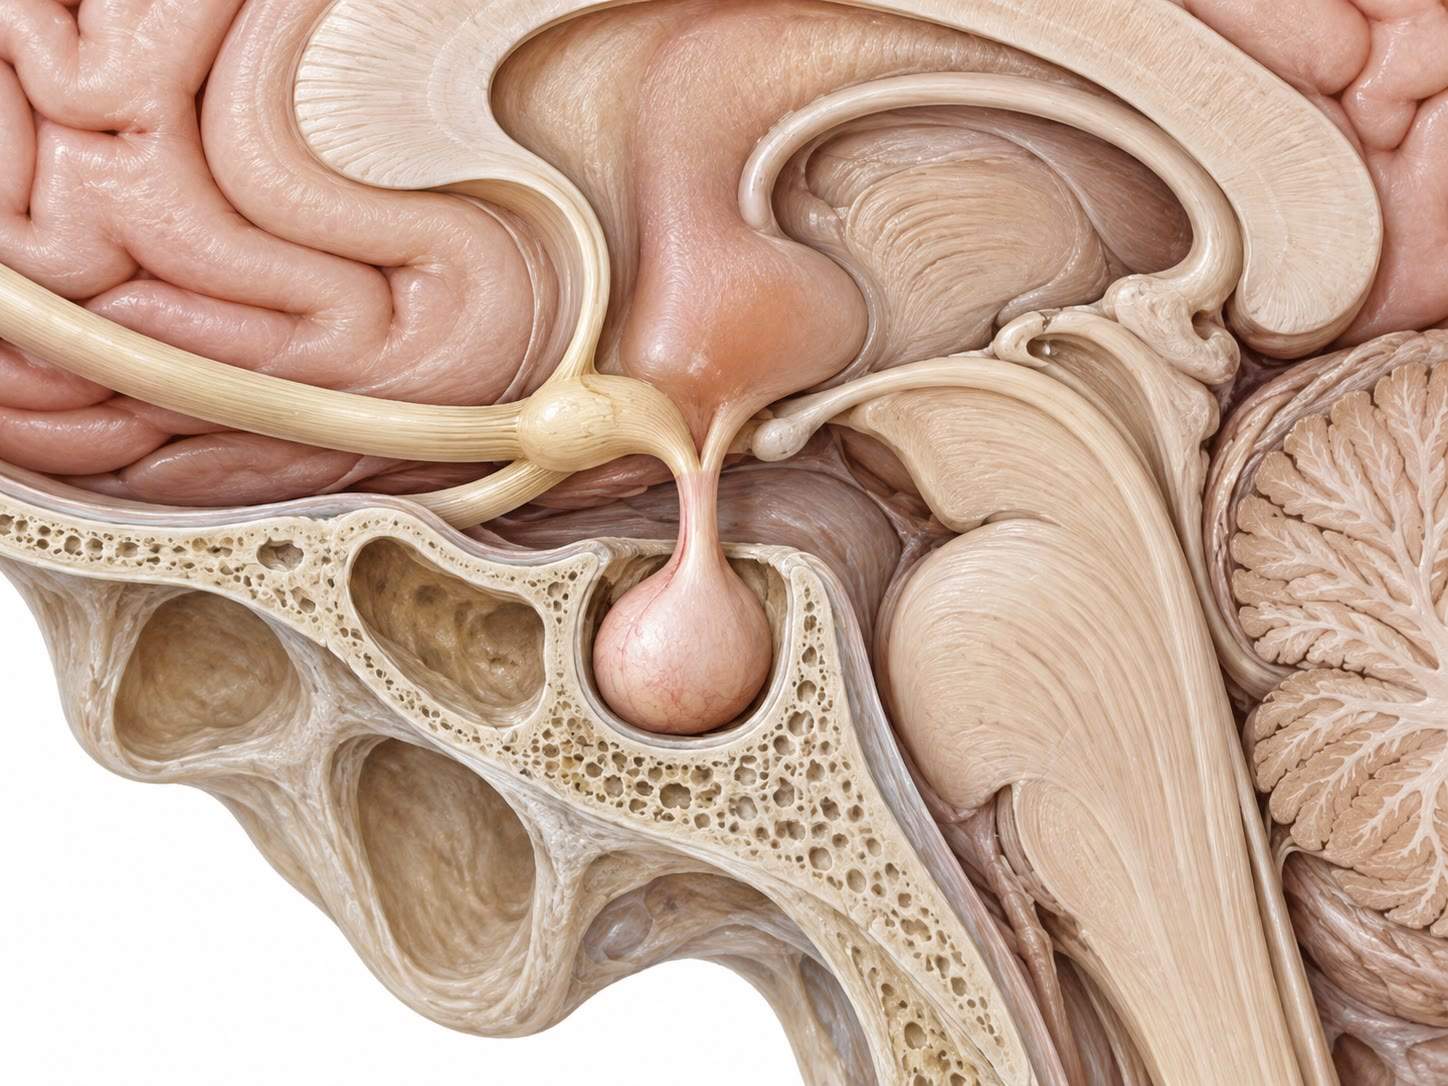
\includegraphics[width=0.55\linewidth]{images/book4/ai/b4-09-hypothalamus-pituitary.jpg}

{\small قاعدة الدماغ في مقطع سهمي: الوطاء
في الأعلى، والساق، والنخامى في جيبها العظمي --- أي
عتاد المحور.}
\end{omfigure}

\section{الذكر: تحكم مقوٍّ}

\begin{proposition}[التحكم في الخصية]\label{prop:b2:reproductive-hormones:testis}
\index{تستوستيرون}\index{إنهيبين}
يؤثر LH في خلايا لايديغ التي تصنع \emph{التستوستيرون}
(\qtyrange{3}{10}{ng/mL} في دم الرجل البالغ، وأكثر بمئة
مرة داخل \omterm{def:b2:mammal-reproduction:testis}{الخصية}). ويؤثر FSH في خلايا سرتولي التي
--- مع التستوستيرون المحلي --- تدعم \omterm{def:b2:mammal-reproduction:testis}{تكوّن النطاف}
وتفرز \emph{الإنهيبين}. ويغذي التستوستيرون راجعًا على الوطاء
والنخامى ليبقي LH منخفضًا؛ ويغذي الإنهيبين راجعًا على النخامى
ليبقي FSH منخفضًا. والحلقتان \emph{سالبتان} والجملة
\emph{مقوّية}: فمستويات الهرمونات تتذبذب مع النبضات ومع
اليوم (وهي أعلاها صباحًا) لكنها لا تدور، وتُصنع النطاف
باستمرار. ويبني التستوستيرون كذلك ويصون الغدد
والقنوات الملحقة، واللحية، والصوت، والعضل والعظم، وإنتاج
الكريات الحمر، والرغبة الجنسية، وهو الذي صنع في الجنين الجسمَ الذكري
(\cref{ch:b2:mammal-reproduction}). والخصاء يزيله: فيرتفع LH و
FSH أضعافًا لانعدام التغذية الراجعة، وتضمر الصفات
الثانوية؛ والتستوستيرون المحقون يعيد الصفات
--- لا الخصوبة، لأنه يكبت أيضًا LH ومن ثم
التستوستيرون داخل \omterm{def:b2:mammal-reproduction:testis}{الخصية} الذي يقتضيه \omterm{def:b2:mammal-reproduction:testis}{تكوّن النطاف}. وهذا
سبب إعقام الستيرويدات البانية الرجالَ.
\end{proposition}
\begin{proof}[شواهد]
خصى برتولد (1849) ديكة: فانكمشت أعرافها ولم تعد
تصيح ولا تتقاتل. أما خصية مطعّمة في بطن
مخصي، حيث نمت لها تروية دموية جديدة لا أعصاب، فأعادت
العرف والصياح والقتال: أي إن \omterm{def:b2:mammal-reproduction:testis}{الخصية} عملت عبر الدم ---
وهو أول برهان على إفراز داخلي، قبل خمسين سنة
من كلمة هرمون. وقد عُزل التستوستيرون واصطُنع سنة 1935.
\end{proof}

\section{الأنثى: دورة بمفتاح}

\begin{definition}[الدورتان المبيضية والرحمية]\label{def:b2:reproductive-hormones:cycle}
\index{دورة طمثية}\index{طور جريبي}\index{طور أصفري}\index{اندفاع LH}\index{بطانة الرحم}
تُعدّ الدورة من أول يوم من الطمث وتدوم
نحو 28 يومًا. \emph{الطور الجريبي} (الأيام 1--14): يجنّد FSH،
وقد تحرر من تغذية \omterm{def:b2:mammal-reproduction:ovary}{الجسم الأصفر} السابق الراجعة بموته، مجموعةً
من الجريبات؛ فتفرز \emph{الإستراديول} الذي يرتفع باطراد؛
ويخفض الإستراديول والإنهيبين FSH، ولا ينجو من الهبوط إلا \omterm{def:b2:mammal-reproduction:ovary}{الجريب}
الأكثر مستقبلات لهرمون FSH --- وهو \omterm{def:b2:mammal-reproduction:ovary}{الجريب} المسيطر. وفي
الرحم، يعيد الإستراديول بناء \emph{بطانة الرحم} (وهو
الطور التكاثري) ويرقّق مخاط عنق الرحم. و\emph{\omterm{def:b2:mammal-reproduction:ovary}{الإباضة}}
(اليوم 14): حين يبقى الإستراديول فوق نحو \qty{200}{pg/mL}
يومًا ونصفًا، تنقلب تغذيته الراجعة على الوطاء والنخامى
من سالبة إلى \emph{موجبة}؛ فيرتفع LH عشرة أضعاف في يوم
--- وهو \emph{اندفاع LH} --- وبعد نحو 36 ساعة من بدايته
ينفجر \omterm{def:b2:mammal-reproduction:ovary}{الجريب} ويطلق البويضة. \emph{والطور الأصفري} (الأيام
15--28): يصير \omterm{def:b2:mammal-reproduction:ovary}{الجريب} المفرَّغ جسمًا أصفر، وهو
تحت LH يفرز \emph{البروجستيرون} (\qtyrange{10}{20}{ng/mL}) و
الإستراديول؛ ويجعل البروجستيرون بطانة الرحم إفرازية، ويثخّن
المخاط، ويرفع حرارة الجسم القاعدية \qty{0.3}{\celsius}،
ويكبت مع الإستراديول LH وFSH. وللجسم الأصفر
عمر نحو 14 يومًا؛ فما لم ينقذه hCG من جنين،
يضمر، ويهبط البروجستيرون والإستراديول، وتنسلخ بطانة الرحم
(\emph{الطمث})، ويرتفع FSH، وتبدأ الدورة التالية. والطور
الأصفري ثابت عند 14 يومًا؛ وإنما التفاوت في طول الدورة
تفاوت في الطور الجريبي.
\end{definition}

\begin{omfigure}
\begin{tikzpicture}
\begin{axis}[
  width=0.94\linewidth, height=6.4cm,
  axis x line=bottom, axis y line=left,
  xmin=0, xmax=28, ymin=0, ymax=1.15,
  xlabel={يوم الدورة}, ylabel={الهرمونات (نسبة إلى الذروة)},
  xlabel style={font=\small, at={(axis description cs:0.5,-0.11)}, anchor=north},
  ylabel style={font=\small},
  tick label style={font=\small}, xtick={0,7,14,21,28}, ytick={0,0.5,1},
  legend style={font=\scriptsize, at={(0.5,-0.25)}, anchor=north, draw=none, legend columns=4},
  clip=false,
]
\addplot[very thick, omThm, domain=0:28, samples=120] {0.1 + 0.9*exp(-((x-14)^2)/0.9)};
\addlegendentry{LH}
\addplot[very thick, omProp, domain=0:28, samples=120] {0.35*exp(-x/6) + 0.15 + 0.35*exp(-((x-14)^2)/1.2)};
\addlegendentry{FSH}
\addplot[very thick, omDef, domain=0:28, samples=160] {0.1 + 0.9*exp(-((x-12.5)^2)/6) + 0.4*exp(-((x-21)^2)/12)};
\addlegendentry{الإستراديول}
\addplot[very thick, omExo!70!black, domain=0:28, samples=160] {0.03 + 0.97*exp(-((x-21)^2)/12)*(x>14)};
\addlegendentry{البروجستيرون}
\draw[dashed, gray] (axis cs:14.5,0) -- (axis cs:14.5,1.1); \node[font=\scriptsize, anchor=south] at (axis cs:14.5,1.1) {الإباضة};
\node[font=\scriptsize, anchor=north] at (axis cs:7,1.1) {الطور الجريبي};
\node[font=\scriptsize, anchor=north] at (axis cs:21.5,1.1) {الطور الأصفري};
\end{axis}
\end{tikzpicture}

{\small هرمونات الدورة. يرتفع الإستراديول من \omterm{def:b2:mammal-reproduction:ovary}{الجريب}
النامي عبر \omterm{def:b2:reproductive-hormones:cycle}{الطور الجريبي}، وبعد عتبة يطلق
\omterm{def:b2:reproductive-hormones:cycle}{اندفاع LH}؛ وتتبعه \omterm{def:b2:mammal-reproduction:ovary}{الإباضة} بعد نحو 36 ساعة؛ ثم
يفرز \omterm{def:b2:mammal-reproduction:ovary}{الجسم الأصفر} البروجستيرون أسبوعين ويموت.}
\end{omfigure}

\begin{omfigure}
\begin{tikzpicture}[every node/.style={font=\scriptsize}]
  % endometrium thickness over the cycle
  \draw[thick, ->] (0,0) -- (12.4,0) node[right] {اليوم};
  \foreach \x/\l in {0/1, 2.1/5, 6.0/14, 12/28} \draw (\x,0.08) -- (\x,-0.08) node[below] {\l};
  \fill[omThm!25] (0,0) -- (0,1.4) .. controls (0.8,1.2) and (1.6,0.5) .. (2.1,0.35) -- (2.1,0) -- cycle;
  \fill[omDef!20] (2.1,0) -- (2.1,0.35) .. controls (3.5,0.6) and (5.2,1.3) .. (6.0,1.5) -- (6.0,0) -- cycle;
  \fill[omExo!35] (6.0,0) -- (6.0,1.5) .. controls (8,1.8) and (11,1.9) .. (12,1.6) -- (12,0) -- cycle;
  \node at (1.0,1.8) {الطمث};
  \node at (4.0,1.8) {التكاثري (الإستراديول)};
  \node at (9,2.2) {الإفرازي (البروجستيرون): غدد، وغليكوجين، وشرايين حلزونية};
  \node[anchor=east] at (-0.1,0.8) {بطانة الرحم};
\end{tikzpicture}

{\small الدورة الرحمية. تنسلخ \omterm{def:b2:reproductive-hormones:cycle}{بطانة الرحم} عند الطمث،
وتُعاد بناءً تحت الإستراديول، وتُجعل إفرازية تحت البروجستيرون،
مستعدةً لاستقبال \omterm{def:b2:mammal-reproduction:implantation}{كيسة أريمية} نحو اليوم 21؛ وحين يهبط
البروجستيرون تنسلخ من جديد.}
\end{omfigure}

\begin{omfigure}
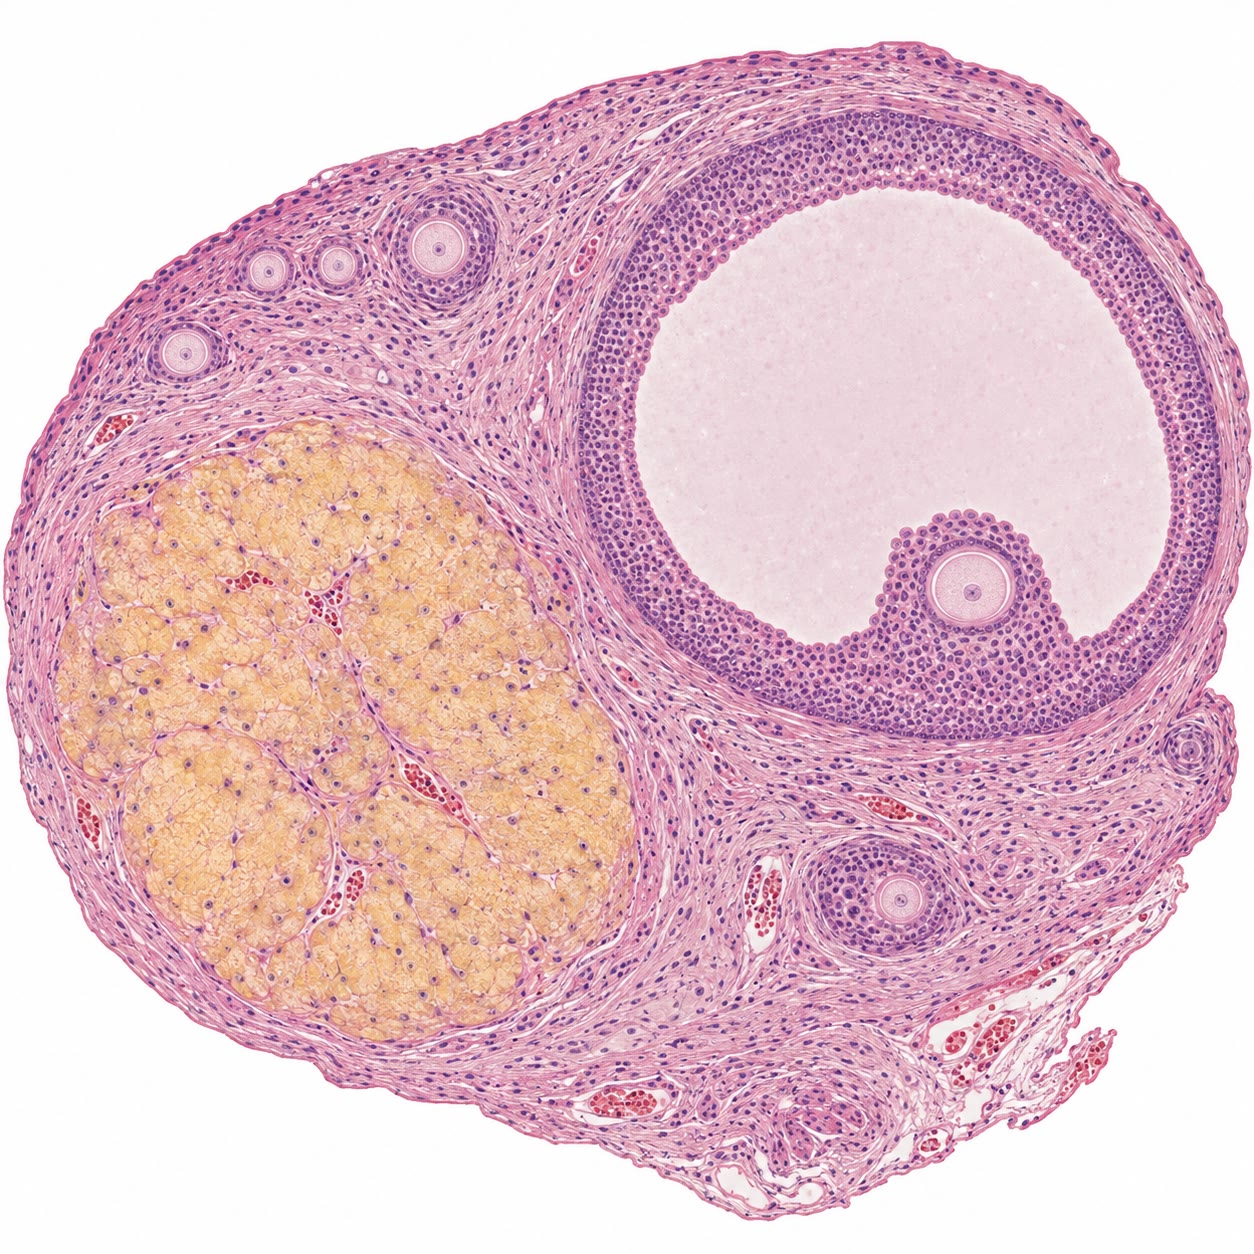
\includegraphics[width=0.46\linewidth]{images/book4/ai/b4-09-ovary-histology.jpg}

{\small مبيض في مقطع: \omterm{def:b2:mammal-reproduction:ovary}{جريب} ناضج بجوفه
وبويضته، وجريبات بدئية صغيرة تحت السطح، \omterm{def:b2:mammal-reproduction:ovary}{وجسم
أصفر} من دورة سابقة.}
\end{omfigure}

\begin{theorem}[الانقلاب من التغذية الراجعة السالبة إلى الموجبة]\label{thm:b2:reproductive-hormones:switch}
\index{تغذية راجعة موجبة!اندفاع LH}
الإستراديول عند المستويات المنخفضة في مطلع \omterm{def:b2:reproductive-hormones:cycle}{الطور الجريبي}
يثبّط LH وFSH؛ أما الإستراديول فوق نحو \qty{200}{pg/mL}، ممسوكًا
أكثر من نحو \qty{36}{h}، فيفعل العكس: إذ يجعل
الوطاء يطلق دفقة من الهرمون المطلق ويجعل النخامى تستجيب لها
بارتفاع عشرة أضعاف في LH. والآلية تغير إشارة لا
تغير مقدار: فالجرعة العالية الممسوكة تستحث في النخامى
مخزونًا كبيرًا من LH وحساسية مرتفعة للهرمون المطلق، وتستحث في
الوطاء (عبر عصبونات الكيسبيبتين) انقلاب مولّد نبضات
الهرمون المطلق إلى نمط الاندفاع. وينقل المفتاح إشارة
متدرجة --- أي كم إستراديولًا يصنع \omterm{def:b2:mammal-reproduction:ovary}{الجريب} --- إلى حدث
كلّي أو معدوم موقوت إلى اليوم، وهو ما تقتضيه
\omterm{def:b2:mammal-reproduction:ovary}{الإباضة}؛ ولأن \omterm{def:b2:mammal-reproduction:ovary}{الجريب} الكبير الناضج وحده يستطيع أن يمسك
\qty{200}{pg/mL}، لا ينطلق الاندفاع إلا حين تكون ثمة بويضة جاهزة
للإطلاق. وحين تقع \omterm{def:b2:mammal-reproduction:ovary}{الإباضة}، يعيد بروجستيرون \omterm{def:b2:mammal-reproduction:ovary}{الجسم
الأصفر} التغذية الراجعة السالبة فلا يتبعها اندفاع ثانٍ.
\end{theorem}
\begin{proof}[شواهد]
عند النساء والقرود اللواتي كُبت المحور عندهن، يتبع تسريبَ
إستراديول يرفع مستوى البلازما فوق \qty{200}{pg/mL}
يومين اندفاعُ LH؛ أما المقدار نفسه معطى يومًا
واحدًا، أو مستوى أدنى ثلاثة أيام، فلا يتبعه. والبروجستيرون المعطى قبل
التسريب يسد الاندفاع؛ والمعطى في الوقت نفسه يقدّمه
ويضخّمه. وعتبة الجرعة والمدة تعيد إنتاج
توقيت الاندفاع الطبيعي من ارتفاع الإستراديول الطبيعي.
\end{proof}

\section{تجاوز الدورة}

\begin{proposition}[الحمل والإرضاع وسن اليأس]\label{prop:b2:reproductive-hormones:overrides}
\index{موجهة الغدد التناسلية المشيمائية البشرية}\index{سن اليأس}
يفرز الجنين المنغرس \emph{hCG}، وهو هرمون شبيه بهرمون LH
يرتبط بمستقبل LH ويبقي \omterm{def:b2:mammal-reproduction:ovary}{الجسم الأصفر} حيًا
مفرزًا بعد أيامه الأربعة عشر؛ وعند الأسبوع العاشر تصنع \omterm{def:b2:mammal-reproduction:placenta}{المشيمة} نفسها
ما يكفي من البروجستيرون والإستروجينات لصون الحمل
ويصير \omterm{def:b2:mammal-reproduction:ovary}{الجسم الأصفر} مستغنى عنه. وطوال الحمل تبقي الستيرويدات
العالية LH وFSH عند الصفر: فلا ينمو \omterm{def:b2:mammal-reproduction:ovary}{جريب} ولا تقع \omterm{def:b2:mammal-reproduction:ovary}{إباضة}.
وبعد الولادة، ترفع الرضاعة البرولاكتين وتبطئ نبضات الهرمون
المطلق، فتبقى \omterm{def:b2:mammal-reproduction:ovary}{الإباضة} مكبوتة أشهرًا. وعند
\emph{\omterm{prop:b2:reproductive-hormones:overrides}{سن اليأس}} ينفد مخزون الجريبات: فيهبط الإستراديول و
الإنهيبين، ولانعدام ما يغذي راجعًا، يرتفع LH وFSH إلى عشرة
أضعاف مستواهما السابق ويبقيان هناك --- وهي بصمة
غدة كفّت عن الجواب.
\end{proposition}

\begin{proposition}[منع الحمل والإنجاب المساعد]\label{prop:b2:reproductive-hormones:clinic}
\index{منع الحمل!هرموني}\index{إلقاح خارج الجسم}
يسلّم القرص المركّب إستروجينًا اصطناعيًا وبروجستينًا
كل يوم: فيبقي مستوى الستيرويد الثابت FSH وLH منخفضين، فلا
يُجنّد \omterm{def:b2:mammal-reproduction:ovary}{جريب}، ولا يقع ارتفاع إستراديول، ولا ينطلق الاندفاع
أبدًا؛ ويثخّن البروجستين كذلك مخاط عنق الرحم. وتدع
فترة الانقطاع التي تدوم سبعة أيام بطانةَ الرحم تنزف؛ وإغفال الأقراص أكثر
من يومين متتاليين يدع FSH يفلت وقد ينمو \omterm{def:b2:mammal-reproduction:ovary}{جريب}.
ومنع الحمل الإسعافي يؤخر الاندفاع أيامًا قليلة بجرعة
بروجستين كبيرة. وفي \emph{\omterm{prop:b2:reproductive-hormones:clinic}{الإلقاح خارج الجسم}} يُقاد المحور
في الاتجاه الآخر: فهرمون FSH يوميًا عشرة أيام يتجاوز
انتقاء \omterm{def:b2:mammal-reproduction:ovary}{جريب} مسيطر واحد وينضج عشرة أو أكثر؛ ويمنع
مضادُّ الهرمون المطلق اندفاعًا تلقائيًا سابقًا لأوانه؛ وتحل حقنة
من hCG محل الاندفاع، وتُجمع البويضات بعد 34
إلى 36 ساعة، قبيل أن تكون قد أُطلقت؛ ثم
تُلقّح في الطبق ويُنقل جنين أو جنينان،
ويُجمّد الباقي. وعند الرجال، يكبت التستوستيرون الخارجي أو نظير
الهرمون المطلق \omterm{def:b2:mammal-reproduction:testis}{تكوّن النطاف} بكبت LH --- وهو مبدأ
مانع حمل هرموني للذكور، لم يُسوَّق بعد. وهذا كله هو
محور القسم الأول، مقروءًا بالمقلوب.
\end{proposition}

\section{تمارين}

\begin{exercise}[$\star$]\label{exo:b2:reproductive-hormones:1}
ارسم المحور عند الذكر: الطبقات الثلاث، والهرمونات الأربعة،
وحلقتي التغذية الراجعة، والخلايا التي يؤثر فيها كل هرمون.
\end{exercise}

\begin{exercise}[$\star$]\label{exo:b2:reproductive-hormones:2}
أعط أطوار الدورتين المبيضية والرحمية بأيامها
وبالهرمون الذي يسود كلًا منها.
\end{exercise}

\begin{exercise}[$\star$]\label{exo:b2:reproductive-hormones:3}
اشرح كيف يمنع القرص المركّب \omterm{def:b2:mammal-reproduction:ovary}{الإباضة}، ولماذا يقع النزف
في أسبوع الانقطاع.
\end{exercise}

\begin{exercise}[$\star$]\label{exo:b2:reproductive-hormones:4}
ماذا يحدث لهرموني LH وFSH وللصفات الجنسية الثانوية عند
ذكر بالغ مخصي؟ وأيها يعكسه التستوستيرون المحقون،
وأيها لا يعكسه؟
\end{exercise}

\begin{exercise}[$\star\star$]\label{exo:b2:reproductive-hormones:5}
تأتي نبضات الهرمون المطلق كل \qty{90}{min} في \omterm{def:b2:reproductive-hormones:cycle}{الطور الجريبي}
وكل \qty{4}{h} في \omterm{def:b2:reproductive-hormones:cycle}{الطور الأصفري}. فكم نبضة في اليوم في كل منهما؟
والنخامى تفضّل LH عند النبضات السريعة وFSH عند البطيئة: فأي
موجهة يجب أن ترتفع أولًا حين يموت \omterm{def:b2:mammal-reproduction:ovary}{الجسم الأصفر}، ولماذا
تكون هي الصحيحة؟
\end{exercise}

\begin{exercise}[$\star\star$]\label{exo:b2:reproductive-hormones:6}
حوّل \qty{200}{pg/mL} من الإستراديول (كتلته المولية
\qty{272}{g/mol}) إلى \unit{pmol/L}، و\qty{15}{ng/mL} من
البروجستيرون (\qty{314}{g/mol}) إلى \unit{nmol/L}. وكم
جزيء إستراديول في ميكرولتر واحد من البلازما عند
عتبة الاندفاع؟
\end{exercise}

\begin{exercise}[$\star\star$]\label{exo:b2:reproductive-hormones:7}
دورات امرأة تدوم 35 يومًا. ولمّا كان \omterm{def:b2:reproductive-hormones:cycle}{الطور الأصفري}
ثابتًا، ففي أي يوم تبيض، وأي الأيام خصيبة إذا
نجت النطاف ثلاثة أيام والبويضة يومًا؟ ولماذا تفشل طريقة
التقويم في الدورات غير المنتظمة؟
\end{exercise}

\begin{exercise}[$\star\star$]\label{exo:b2:reproductive-hormones:8}
ينغرس جنين في اليوم 21 من دورة طولها 28 يومًا، ويبدأ hCG عنده
عند \qty{1}{IU/L} ويتضاعف كل يومين. ويحتاج \omterm{def:b2:mammal-reproduction:ovary}{الجسم الأصفر} إلى
بضع وحدات دولية في اللتر من hCG بحلول اليوم 26 لينجو. فهل الجنين في الوقت؟ وماذا
كان ليحدث لو تأخر \omterm{def:b2:mammal-reproduction:implantation}{الانغراس} إلى اليوم 25؟
\end{exercise}

\begin{exercise}[$\star\star$]\label{exo:b2:reproductive-hormones:9}
اذكر ما بيّنته تجربة كنوبيل وما استبعدته، و
تنبّأ بأثر إعطاء امرأة ناهضًا طويل الأثر للهرمون المطلق
شهرًا: على LH، وعلى الإستراديول، وعلى \omterm{def:b2:reproductive-hormones:cycle}{بطانة الرحم}.
\end{exercise}

\begin{exercise}[$\star\star\star$]\label{exo:b2:reproductive-hormones:10}
في نموذج المستقبلات، خذ $s = 100$ مستقبل في الساعة، و$d =
\qty{0.5}{h^{-1}}$، و$iH = \qty{6}{h^{-1}}$ ما دام الهرمون
حاضرًا. احسب عدد المستقبلات في الحالة المستقرة بلا هرمون
ومع هرمون مستمر. ومع نبضة مدتها دقيقتان كل ساعة،
احسب العدد المفقود في النبضة وكسر العجز
المستعاد قبل النبضة التالية، واستنتج المستوى الذي
يستقر حوله المخزون.
\end{exercise}

\begin{exercise}[$\star\star\star$]\label{exo:b2:reproductive-hormones:11}
امرأة بعد \omterm{prop:b2:reproductive-hormones:overrides}{سن اليأس} عندها LH وFSH بعشرة أضعاف مستواهما عند امرأة
شابة وإستراديول منخفض جدًا؛ وامرأة بورم نخامي
يفرز البرولاكتين عندها LH منخفض وإستراديول منخفض ولا دورات؛
وامرأة بورم في الخلايا الحُبيبية عندها إستراديول عالٍ وLH منخفض
ولا دورات. اشرح كل نميط انطلاقًا من المحور.
\end{exercise}

\begin{exercise}[$\star\star\star$]\label{exo:b2:reproductive-hormones:12}
«الهرمون نفسه يثبّط \omterm{def:b2:reproductive-hormones:cycle}{اندفاع LH} ثم يطلقه.»
اشرح كيف يكون للإستراديول الأثران معًا، ولماذا تحتاج \omterm{def:b2:mammal-reproduction:ovary}{الإباضة} إلى
مفتاح لا إلى مقياس متدرج، وما الذي كان ليختل مع المقياس المتدرج.
\end{exercise}

\section{مسألة: دورة مقيسة}

\begin{problem}[{مسألة نهاية الأسبوع --- قياسات هرمونية يومية لدورة
واحدة تُقرأ لأطوارها ويوم الإباضة والنافذة الخصيبة؛ وتُحسب عتبة
الاندفاع وساعة الجسم الأصفر وإنقاذ hCG؛ ويشرح نموذج المستقبلات
تجربة كنوبيل؛ ويُقاد المحور بالمقلوب في العيادة، وتنتهي إلى يوم
الإباضة وطول الطور الأصفري والنافذة الخصيبة وعتبة الاندفاع}]
\label{pb:b2:reproductive-hormones:1}
أُخذت عينات دم في أيام مختارة من دورة امرأة:

\begin{center}
\small
\begin{tabular}{lcccccccccc}
\hline
اليوم & 1 & 5 & 8 & 11 & 12 & 13 & 14 & 15 & 21 & 27 \\
\hline
الإستراديول (\unit{pg/mL}) & 40 & 60 & 110 & 210 & 260 & 310 & 220 & 150 & 160 & 50 \\
LH (\unit{IU/L}) & 5 & 5 & 6 & 7 & 8 & 20 & 65 & 15 & 4 & 4 \\
البروجستيرون (\unit{ng/mL}) & 0.5 & 0.5 & 0.6 & 0.7 & 0.8 & 1.0 & 1.5 & 3 & 16 & 2 \\
الحرارة (\unit{\celsius}) & 36.4 & 36.4 & 36.4 & 36.4 & 36.4 & 36.4 & 36.4 & 36.5 & 36.8 & 36.7 \\
\hline
\end{tabular}
\end{center}

بدأ الطمث في اليوم 1 وبدأ من جديد في اليوم 29.

\medskip
\noindent\textbf{الجزء الأول --- قراءة الدورة.}
\begin{enumerate}
  \item عيّن الطورين الجريبي والأصفري من الجدول،
        مع الهرمون الذي يعلّم كلًا منهما.
  \item في أي يوم بلغ \omterm{def:b2:reproductive-hormones:cycle}{اندفاع LH} ذروته؟ ومتى وقعت \omterm{def:b2:mammal-reproduction:ovary}{الإباضة}؟
  \item كم دام \omterm{def:b2:reproductive-hormones:cycle}{الطور الأصفري}؟ وهل ذلك متسق مع عمر
        \omterm{def:b2:mammal-reproduction:ovary}{الجسم الأصفر}؟
  \item اشرح انزياح الحرارة ولماذا يؤكد \omterm{def:b2:mammal-reproduction:ovary}{الإباضة} ولا
        يستطيع التنبؤ بها.
  \item في أي الأيام كان الإستراديول فوق \qty{200}{pg/mL}؟ واربط
        المدة بالاندفاع.
  \item أعط النافذة الخصيبة لهذه الدورة (النطاف ثلاثة أيام،
        والبويضة يوم).
\end{enumerate}

\medskip
\noindent\textbf{الجزء الثاني --- الأرقام.}
\begin{enumerate}[resume]
  \item حوّل إستراديول اليوم 13 إلى \unit{pmol/L}، وبروجستيرون
        اليوم 21 إلى \unit{nmol/L}.
  \item بأي عامل ارتفع LH من اليوم 12 إلى اليوم 14؟ ولماذا
        يهبط بهذه السرعة بعد ذلك (وعمر النصف لهرمون LH نحو
        \qty{1}{h})؟
  \item لو كان لدورة هذه المرأة التالية \omterm{def:b2:reproductive-hormones:cycle}{طور جريبي} طوله 21 يومًا،
        ففي أي يوم تبيض وكم يكون طول الدورة؟
  \item ينغرس جنين بعد 7 أيام من \omterm{def:b2:mammal-reproduction:ovary}{الإباضة}. ففي أي يوم من هذه
        الدورة يظهر hCG، وإذا تضاعف كل يومين
        من \qty{1}{IU/L}، فأي مستوى يبلغ بحلول اليوم 27؟
  \item اشرح لماذا يبين بروجستيرون اليوم 27 البالغ \qty{2}{ng/mL}
        أنه لم ينغرس جنين.
  \item أي قيمتين للبروجستيرون والإستراديول كانتا ستُقرآن في
        اليوم 27 لو انغرس جنين؟
\end{enumerate}

\medskip
\noindent\textbf{الجزء الثالث --- التغذية الراجعة والنبضات.}
\begin{enumerate}[resume]
  \item اشرح، بإشارات التغذية الراجعة، لماذا يكون FSH أعلى ما
        يكون في مطلع الدورة ولماذا لا ينجو عادةً إلا \omterm{def:b2:mammal-reproduction:ovary}{جريب}
        واحد.
  \item في نموذج المستقبلات مع $s = 100$ في الساعة، و$d =
        \qty{0.5}{h^{-1}}$، و$iH = \qty{6}{h^{-1}}$، احسب $R^*$
        بلا هرمون وتحت هرمون مستمر.
  \item تدوم النبضة \qty{2}{min}. فانطلاقًا من $R^*$ غير
        المنبَّه، كم مستقبلًا تزيل نبضة واحدة (استعمل
        التقريب الخطي $iHR\,\Delta t$)؟ وأي كسر من
        العجز يُستعاد في الساعة التي قبل النبضة التالية
        (بثابت زمن $1/d$)، وحول أي مستوى يستقر
        المخزون؟
  \item استعمل هذه الأرقام لشرح نتيجة كنوبيل.
  \item يُعطى رجل ناهضًا للهرمون المطلق باستمرار من أجل سرطان
        الموثة. تنبّأ بهرمون LH وبالتستوستيرون عنده بعد يوم
        وبعد شهر، واشرح الفرق.
  \item خلايا الحُبيبية عند امرأة لا تصنع الإنهيبين. تنبّأ
        بهرموني FSH وLH عندها، وبالعاقبة على تجنيد الجريبات.
\end{enumerate}

\medskip
\noindent\textbf{الجزء الرابع --- العيادة.}
\begin{enumerate}[resume]
  \item من أجل \omterm{prop:b2:reproductive-hormones:clinic}{الإلقاح خارج الجسم} تتلقى هذه المرأة FSH يوميًا
        من اليوم 2. اشرح لماذا ينضج عشرة جريبات بدل واحد.
  \item لماذا يُضاف مضادٌّ للهرمون المطلق من اليوم 6، وماذا كان
        ليحدث دونه؟
  \item يُحقن hCG حين تنضج الجريبات؛ وتُجمع البويضات
        بعد 35 ساعة. برهن على التوقيت من الجدول.
  \item تُجمع عشر بويضات؛ فتُلقّح \qty{70}{\%} منها، وتبلغ
        \qty{40}{\%} من الأجنة طور \omterm{def:b2:mammal-reproduction:implantation}{الكيسة الأريمية}، وتنغرس كل
        كيسة منقولة باحتمال $0.35$.
        فما العدد المنتظر للكيسات الأريمية؟ وما احتمال حمل واحد
        على الأقل إذا نُقلت كيستان؟
  \item اشرح لماذا كان القرص المركّب، لو تناولته هذه المرأة،
        ليعطي جدولًا بلا \omterm{def:b2:reproductive-hormones:cycle}{اندفاع LH} وبلا ارتفاع بروجستيرون.
  \item مانع حمل ذكري قائم على مضادٍّ للهرمون المطلق سيلغي
        التستوستيرون أيضًا. فما الذي يجب إعطاؤه معه، ولماذا
        لا يعيد إعطاؤه إنتاج النطاف؟
  \item اذكر النتيجة: يوم \omterm{def:b2:mammal-reproduction:ovary}{الإباضة}، وطول \omterm{def:b2:reproductive-hormones:cycle}{الطور الأصفري}، والنافذة
        الخصيبة، وعتبة الإستراديول ومدتها اللتان أطلقتا الاندفاع.
\end{enumerate}
\end{problem}
